% =====================================================================
%  Face Reconstruction with PCA: Efficiency and Effectiveness Analysis
%  IEEEtran two-column paper. Numbers are macros generated by build.py
%  from the experiment console output (single source of truth).
% =====================================================================
% 明确指定正文与数学字体，避免 XeTeX 将 IEEE 的 Times 字体静默回退。
\RequirePackage[T1]{fontenc}
\documentclass[journal]{IEEEtran}

\usepackage{mathptmx}
\usepackage{amsmath,amssymb}
\usepackage{graphicx}
\usepackage{booktabs}
\usepackage{multirow}
\usepackage{url}
% 自动平衡末页双栏，兼容 Times 字体的行深度及参考文献标题。
\usepackage{flushend}
\usepackage{float}
\usepackage{tikz}
\usetikzlibrary{positioning,arrows.meta,calc,fit}
\usepackage[hidelinks]{hyperref}

\graphicspath{{figs/}}

\definecolor{myblue}{RGB}{30,79,168}
\definecolor{myred}{RGB}{200,60,50}
\definecolor{mygray}{RGB}{110,120,130}

% ---- float placement quotas (see delivery checklist) ----
\renewcommand{\topfraction}{0.92}
\renewcommand{\bottomfraction}{0.85}
\renewcommand{\textfraction}{0.06}
\renewcommand{\floatpagefraction}{0.78}
\setcounter{topnumber}{2}
\setcounter{dbltopnumber}{2}
\renewcommand{\dbltopfraction}{0.85}
\setcounter{totalnumber}{3}

\setlength{\emergencystretch}{1em}
\setlength{\floatsep}{12pt plus 3pt minus 2pt}
\setlength{\textfloatsep}{14pt plus 3pt minus 2pt}
\setlength{\intextsep}{12pt plus 3pt minus 2pt}
% 浮动页从顶部排起，避免图表间的弹性留白被放大。
\makeatletter
\setlength{\@fptop}{0pt}
\setlength{\@fpsep}{12pt plus 2pt minus 2pt}
\setlength{\@fpbot}{0pt plus 1fil}
\setlength{\@dblfptop}{0pt}
\setlength{\@dblfpsep}{12pt plus 2pt minus 2pt}
\setlength{\@dblfpbot}{0pt plus 1fil}
\makeatother

% auto-generated by build.py from results/console_output.txt — do not edit by hand
\newcommand{\nN}{400}
\newcommand{\nDim}{4096}
\newcommand{\nK}{20}
\newcommand{\nVarKsSum}{76.34\%}
\newcommand{\nCompRatio}{0.49\%}
\newcommand{\nMSEBase}{0.01927}
\newcommand{\nMSEK}{0.00456}
\newcommand{\nPSNRK}{23.640}
\newcommand{\nDrop}{76.3\%}
\newcommand{\nPredK}{0.004571}
\newcommand{\nObsK}{0.004559}
\newcommand{\nRelDev}{0.25\%}
\newcommand{\nSsimK}{0.698}
\newcommand{\nAccK}{94.8\%}
\newcommand{\nAccSat}{95.5\%}
\newcommand{\nSepPix}{0.675}
\newcommand{\nSepPCA}{0.562}
\newcommand{\nWithinPix}{8.3777}
\newcommand{\nBetweenPix}{12.4144}
\newcommand{\nWithinPCA}{6.0258}
\newcommand{\nBetweenPCA}{10.7313}
\newcommand{\nEqDiff}{$1.97\times10^{-7}$}
\newcommand{\nSvdMed}{0.97}
\newcommand{\nSvdLow}{0.82}
\newcommand{\nSvdHigh}{1.43}
\newcommand{\nEighMed}{23.4}
\newcommand{\nEighLow}{21.4}
\newcommand{\nEighHigh}{24.7}
\newcommand{\nSvdMedTwo}{1.22}
\newcommand{\nEighMedTwo}{20.4}
\newcommand{\nSpeedup}{24}
\newcommand{\nMSEstd}{0.00150}
\newcommand{\nCovMem}{134\,MB}
\newcommand{\nStorageOrig}{13.1\,MB}
\newcommand{\nStorageKB}{64\,kB}
\newcommand{\nCompress}{205}

\newcommand{\nTrainN}{280}
\newcommand{\nTestN}{120}
\newcommand{\nTestMSE}{0.00538}
\newcommand{\nTestPSNR}{22.962}
\newcommand{\nTestSSIM}{0.654}
\newcommand{\nTestAcc}{89.2\%}
\newcommand{\nTestAccCI}{5.6}
\newcommand{\nTestSep}{0.559}
\newcommand{\nSsimBase}{0.451}
\newcommand{\nSsimGain}{0.247}
\newcommand{\nLatency}{0.03}
\newcommand{\nMseRise}{17.9\%}


\begin{document}

\title{PCA Face Reconstruction on the Olivetti Dataset:\\
Quality and Computational Efficiency}

\author{Weixin Chen\\
\small Course Project, Big Data Analysis and Processing\\
\small Nanjing University of Posts and Telecommunications}

\maketitle

\begin{abstract}
Principal component analysis (PCA) provides compact face representations,
but selecting a practical configuration requires assessing reconstruction
quality and computational cost together. This study evaluates a PCA pipeline
on the Olivetti dataset of $\nN$ grayscale images with $\nDim$ pixels each.
Covariance eigendecomposition and economy singular value decomposition
(SVD) are compared using reconstruction, structural, classification, and
resource metrics. With $k=\nK$ components, PCA retains \nVarKsSum{} of the
variance and reduces mean squared error from \nMSEBase{} to \nMSEK{}.
The structural similarity index reaches \nSsimK{}, while self-excluded
nearest-neighbor classification achieves \nAccK{} accuracy using a basis
fitted to all images. The within-/between-subject distance ratio decreases
from \nSepPix{} in pixel space to \nSepPCA{} in PCA space. A fixed
\nTrainN/\nTestN{} split yields test error \nTestMSE{} and accuracy
\nTestAcc{} on unseen images of the same subjects. Economy SVD produces
numerically equivalent reconstructions while reducing median decomposition
time from \nEighMed{} to \nSvdMed{}\,s on the tested machine. Coefficient
storage requires \nStorageKB{}, excluding the shared basis and mean,
compared with \nStorageOrig{} for the original float64 data. These results
characterize the quality--cost trade-off of an established linear baseline
and show why component selection should reflect the intended task.
\end{abstract}

\begin{IEEEkeywords}
Eigenfaces, face reconstruction, principal component analysis, singular value decomposition,
structural similarity.
\end{IEEEkeywords}

\section{Introduction}
\IEEEPARstart{A}{} grayscale face image with $64\times64$ pixels contains
$d=\nDim$ values, many of which are correlated. A compact representation
can reduce storage and processing costs while preserving information useful
for reconstruction and identity classification. Pixel-space distances also
reflect changes in illumination, expression, and pose. Reconstruction error
alone therefore provides an incomplete assessment of a face representation.

PCA finds orthogonal directions of maximal variance and reconstructs images
from the retained components~\cite{jolliffe}. Its eigenface interpretation
connects dimensionality reduction with appearance-based face
representation~\cite{turk}. Choosing a component count and choosing a solver
address different requirements: the former controls retained information,
whereas the latter determines the cost of estimating the same subspace.

This study examines both choices on the Olivetti face
database~\cite{orl,sklearn}. A from-scratch implementation compares
covariance eigendecomposition with economy SVD and checks their numerical
agreement. Reconstruction is assessed using mean squared error (MSE), peak
signal-to-noise ratio (PSNR), and structural similarity (SSIM). Identity
information is assessed using one-nearest-neighbor (1-NN) classification
and within-/between-subject distances. Runtime measurements complement
complexity and storage estimates, while a held-out split evaluates images
excluded from basis estimation. Together, these analyses relate component
and solver choices to the quality and cost of this linear baseline.

\section{Methods}

\subsection{PCA Formulation}
Let $X\in\mathbb{R}^{n\times d}$ hold one face per row and
$\mu=\frac1n\sum_i x_i$ be the mean face. After centering,
$\tilde X = X-\mathbf{1}\mu^{\!\top}$, PCA solves
\begin{equation}
C\,v_j=\lambda_j v_j,\qquad
C=\frac{1}{n-1}\tilde X^{\!\top}\tilde X ,
\label{eq:eig}
\end{equation}
with eigenvalues sorted in descending order. Keeping the leading $k$
eigenvectors as $W=[v_1,\dots,v_k]\in\mathbb{R}^{d\times k}$ gives the code
and the linear reconstruction
\begin{equation}
z = W^{\!\top}(x-\mu),\qquad
\hat x = \mu + W z = \mu + \sum_{j=1}^{k} z_j v_j .
\label{eq:proj}
\end{equation}
The explained-variance ratio is
$\eta_j=\lambda_j/\sum_{i=1}^{d}\lambda_i$~\cite{abdi}.
The denominator includes the full spectrum; normalizing only over retained
components would overstate variance retention. Centering limits the rank
of $\tilde X$ to at most $n-1$.

Each eigenvector, reshaped to $64\times64$, is an \emph{eigenface}: the
leading components show broad intensity patterns, while later components
show more localized variation (Fig.~\ref{fig:eigenfaces}). The complete
pipeline is summarized in Fig.~\ref{fig:pipeline}.

\begin{figure*}[t]
  \centering
  \resizebox{\textwidth}{!}{%
  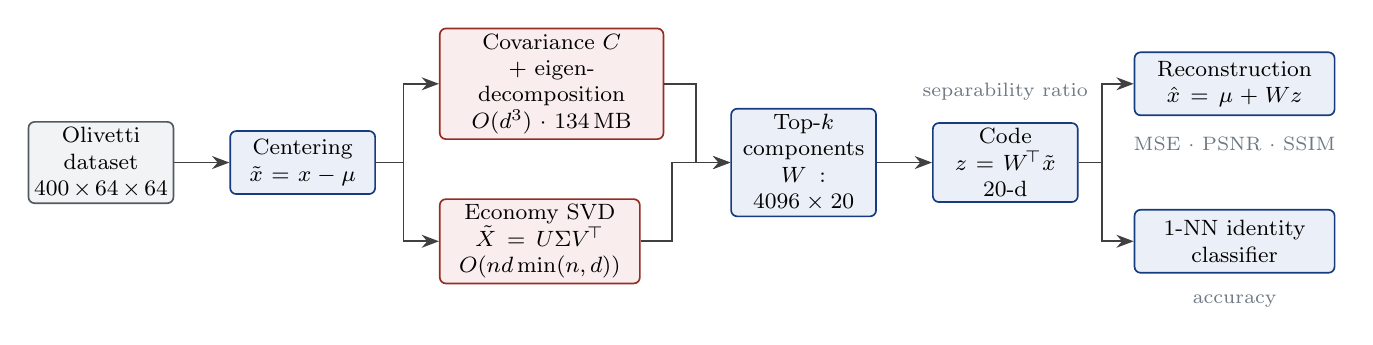
\begin{tikzpicture}[
    font=\footnotesize,
    box/.style={draw=#1!75!black, fill=#1!9, rounded corners=2.2pt,
                line width=0.6pt, minimum height=8mm, text width=17mm,
                align=center, inner sep=2pt},
    arr/.style={-{Stealth[length=2.2mm]}, line width=0.6pt, draw=black!75},
    lab/.style={font=\scriptsize, text=mygray},
  ]
    \node[box=mygray] (data) {Olivetti dataset\\$400\times64\times64$};
    \node[box=myblue, right=7mm of data] (center) {Centering\\$\tilde x = x-\mu$};
    \node[box=myred, text width=27mm, right=8mm of center, yshift=10mm] (cov) {Covariance $C$\\$+$ eigen-decomposition\\$O(d^{3})$ $\cdot$ \nCovMem};
    \node[box=myred, text width=24mm, right=8mm of center, yshift=-10mm] (svd) {Economy SVD\\$\tilde X=U\Sigma V^{\!\top}$\\$O(nd\min(n,d))$};
    \node[box=myblue, right=45mm of center] (topk) {Top-$k$ components\\$W: 4096\times20$};
    \node[box=myblue, right=7mm of topk] (code) {Code $z=W^{\!\top}\tilde x$\\20-d};
    \node[box=myblue, text width=24mm, right=7mm of code, yshift=10mm] (recon) {Reconstruction\\$\hat x=\mu+Wz$};
    \node[box=myblue, text width=24mm, right=7mm of code, yshift=-10mm] (knn) {1-NN identity\\classifier};

    \draw[arr] (data) -- (center);
    \draw[arr] (center.east) -- ++(0.35,0) |- (cov.west);
    \draw[arr] (center.east) -- ++(0.35,0) |- (svd.west);
    \draw[arr] (cov.east) -- ++(4mm,0) |- (topk.west);
    \draw[arr] (svd.east) -- ++(4mm,0) |- (topk.west);
    \draw[arr] (topk) -- (code);
    \draw[arr] (code.east) -- ++(0.3,0) |- (recon.west);
    \draw[arr] (code.east) -- ++(0.3,0) |- (knn.west);

    % 求解器等价关系已在正文公式中给出，避免公式标签与分支连线相交。

    \node[lab, below=1.5mm of recon] {MSE $\cdot$ PSNR $\cdot$ SSIM};
    \node[lab, below=1.5mm of knn] {accuracy};
    \node[lab, above=1.5mm of code] {separability ratio};
  \end{tikzpicture}}
  \caption{PCA pipeline at $k=20$. The two decomposition routes estimate the
  same principal subspace. The covariance storage label assumes float64;
  runtime and array storage are compared in Table~\ref{tab:eff}.}
  \label{fig:pipeline}
\end{figure*}

\begin{figure*}[t]
  \centering
  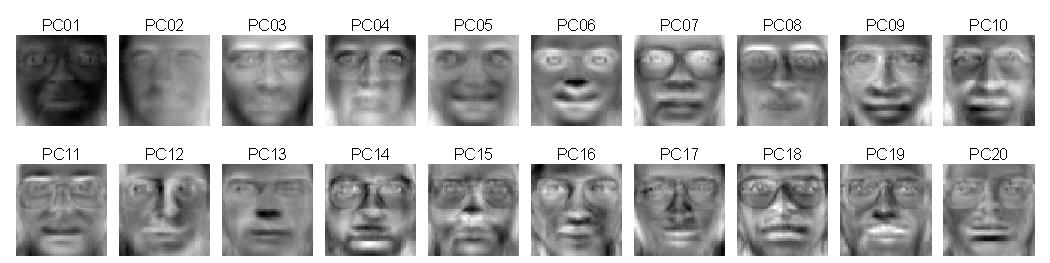
\includegraphics[width=\textwidth]{fig2_eigenfaces.pdf}
  \caption{The first 20 eigenfaces (PC01--PC20, in descending order of
  eigenvalue). Each component is displayed with its own symmetric intensity
  scale to reveal spatial patterns; sign and display contrast do not indicate
  component importance.}
  \label{fig:eigenfaces}
\end{figure*}

\subsection{Two Equivalent Solvers and Their Cost}
\emph{Covariance route.} Form $C\in\mathbb{R}^{d\times d}$ explicitly and
eigendecompose it, \eqref{eq:eig}. Forming $C$ costs $O(nd^2)$ and its
eigendecomposition $O(d^3)$; the matrix itself occupies $d^2$ doubles.
\emph{SVD route.} Decompose the centered data directly,
$\tilde X=U\Sigma V^{\!\top}$. Since
$\tilde X^{\!\top}\tilde X=V\Sigma^2V^{\!\top}$, the columns of $V$ are the
eigenvectors in \eqref{eq:eig} and
\begin{equation}
\lambda_j=\sigma_j^2/(n-1),
\label{eq:svd}
\end{equation}
so the two routes are algebraically identical, while the economy SVD costs
$O(nd\min(n,d))$ and never materializes $C$~\cite{golub}. A third variant,
the Gram-matrix trick ($\tilde X\tilde X^{\!\top}\in\mathbb{R}^{n\times n}$,
eigendecompose, recover $V=\tilde X^{\!\top}U\Sigma^{-1}$), costs
$O(n^2d+n^3)$ when restricted to nonzero singular values. This variant is
outside the timing comparison. Linear variants such as
two-dimensional PCA~\cite{yang} and nonlinear kernel PCA~\cite{scholkopf}
extend the variance-ordering principle; the present comparison focuses on
the standard linear formulation.

\subsection{Evaluation Metrics}
\label{sec:design}
\emph{Reconstruction.} For image $i$,
$\mathrm{MSE}_i=d^{-1}\|x_i-\hat x_i\|_2^2$ and
$\mathrm{PSNR}_i=10\log_{10}(1/\mathrm{MSE}_i)$ for unit-range pixels.
Both metrics are averaged over images, so mean PSNR is not computed from
the aggregate MSE. Structural similarity~\cite{ssim} is
\begin{equation}
\mathrm{SSIM}(x,\hat x)=
\frac{(2\mu_x\mu_{\hat x}+c_1)(2\sigma_{x\hat x}+c_2)}
{(\mu_x^2+\mu_{\hat x}^2+c_1)(\sigma_x^2+\sigma_{\hat x}^2+c_2)} .
\label{eq:ssim}
\end{equation}
Here $\mu_x$, $\sigma_x^2$, and $\sigma_{x\hat x}$ denote local means,
variances, and covariance, and $c_1,c_2$ stabilize the ratios. We use
scikit-image's \texttt{structural\_similarity} function with unit data range
and otherwise retain its default settings, then average the image scores.

\emph{Identity information.} Euclidean 1-NN classification is evaluated on
40 identities without tuning. In the full-data evaluation, PCA is fitted
once to all images and each query is excluded from its own neighbor search.
This is a self-excluded evaluation with a fixed basis, not cross-validation
that refits PCA for every query. Separability is summarized by the ratio of
mean within-subject to mean between-subject distances; a lower ratio means
smaller within-subject distances relative to between-subject distances.

\emph{Resources.} Decomposition time is the median of three wall-clock
runs on one machine. Complexity, array storage, and coefficient storage are
analyzed separately. Array sizes assume eight bytes per element and are
reference float64 estimates, not measured process peak memory.

\section{Experimental Setup}
The scikit-learn version of the Olivetti face
dataset~\cite{orl,sklearn} contains $n=\nN$ grayscale images of
$64\times64$ pixels from 40 subjects (ten images each), with pixel values
normalized to $[0,1]$. The pipeline of
Fig.~\ref{fig:pipeline} is implemented in Python with NumPy and
Matplotlib, with the random seed fixed at zero so that the sampled image
(index 172, subject 17) and all figures are reproducible. Unless stated
otherwise, $k=\nK$ matches the course requirement; sweeps use
$k\in\{5,10,20,50,100\}$ for quality and
$\{5,10,20,30,50,66,100,150\}$ for accuracy. Both solvers are implemented and
cross-checked: the reconstructions agree to a maximum absolute difference of
\nEqDiff{}, and the reported explained variance agrees. The original
timing routine uses centered float32 input; float64 storage estimates
are reported independently of that benchmark. For the held-out check, the
first seven images of each subject form the training set and the last three
form the test set. The training mean and basis are estimated without test
images, and training projections serve as the 1-NN gallery.

% 提前声明宽幅结果图，使其紧邻首次讨论所在页面。
\begin{figure*}[t]
  \centering
  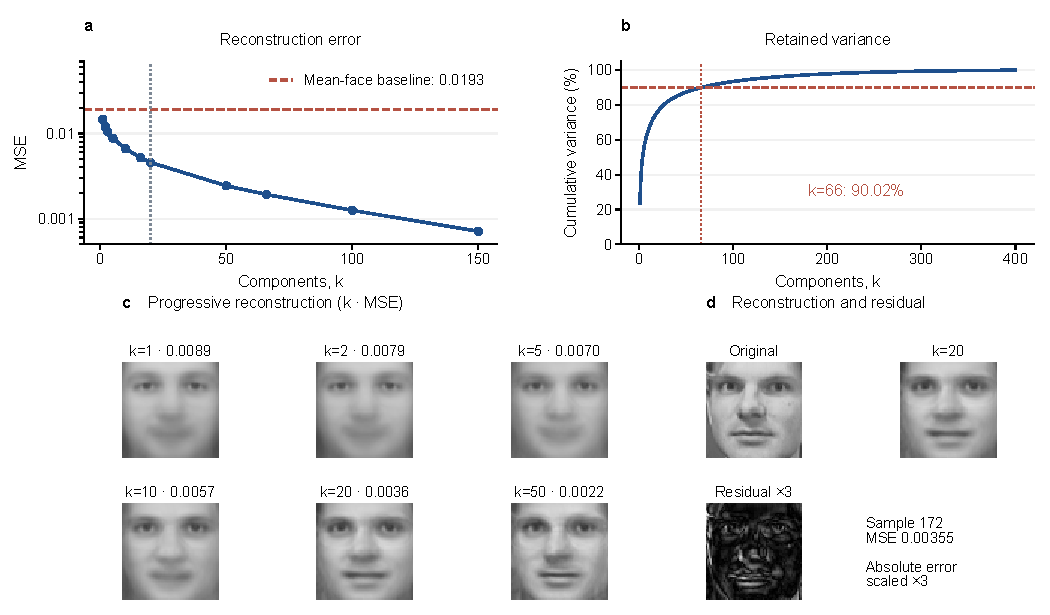
\includegraphics[width=\textwidth]{fig4_results_dashboard.pdf}
  \caption{Effectiveness at a glance. (a) Reconstruction error versus $k$
  (log scale) with the mean-face baseline and the $k=20$ operating point;
  (b) full-spectrum cumulative explained variance, marking $k=66$ where 90\%
  is reached; (c) cumulative reconstructions of the sampled face for
  $k=1,2,5,10,20,50$ with per-panel MSE; (d) the same face, its $k=20$
  reconstruction and the $3\times$ amplified residual, which concentrates on
  edges and high-frequency structures.}
  \label{fig:results}
\end{figure*}

\section{Results}

\subsection{Reconstruction Quality}
Fig.~\ref{fig:results}(a) and Table~\ref{tab:k} summarize the
quality--complexity trade-off. Relative to the mean-face baseline (\nMSEBase{}), $k=\nK$ reduces
the MSE to \nMSEK{} (a \nDrop{} reduction), with mean PSNR
\nPSNRK{}\,dB. Per-image MSE is \nMSEK{} $\pm$ \nMSEstd{}
(mean $\pm$ standard deviation). SSIM increases from \nSsimBase{} for the
mean-face baseline to \nSsimK{} at $k=\nK$.

The discarded eigenvalues determine the full-data reconstruction error:
\begin{equation}
\mathrm{MSE}_k=\frac{\|\tilde X-\tilde XWW^{\!\top}\|_F^2}{nd}
=\frac{n-1}{nd}\sum_{j>k}\lambda_j.
\label{eq:mse}
\end{equation}
The factor $(n-1)/n$ reconciles sample-covariance normalization with
per-pixel MSE. The original log reports the uncorrected value
$\sum_{j>k}\lambda_j/d=\nPredK{}$ versus observed \nObsK{}.
Its \nRelDev{} relative difference is accounted for by this normalization
factor, rather than a solver discrepancy.

\begin{table}[!t]
  \caption{Full-sample reconstruction quality. PSNR and SSIM are
  averaged over images; $k=0$ uses the mean face.}
  \label{tab:k}
  \centering
  \footnotesize
  \setlength{\tabcolsep}{7pt}
  \begin{tabular}{@{}lrrr@{}}
    \toprule
    $k$ & MSE & PSNR (dB) & SSIM \\
    \midrule
    0 (mean face) & 0.01927 & 17.516 & 0.451 \\
    5 & 0.00879 & 20.798 & 0.540 \\
    10 & 0.00662 & 22.036 & 0.615 \\
    \textbf{20} & \textbf{0.00456} & \textbf{23.640} & \textbf{0.698} \\
    50 & 0.00243 & 26.359 & 0.812 \\
    100 & 0.00125 & 29.182 & 0.888 \\
    \bottomrule
  \end{tabular}
\end{table}




Reaching 90\% variance retention requires $k=66$, compared with
\nVarKsSum{} at $k=\nK$. The cumulative reconstructions in
Fig.~\ref{fig:results}(c) show the recovery of finer facial structure as $k$
increases. For the illustrated image, the residual in
Fig.~\ref{fig:results}(d) is prominent near facial boundaries, glasses, and
the hairline, indicating detail lost at the selected component count.

\subsection{Identity Separability and Classification}
\label{sec:separation}
Fig.~\ref{fig:metrics}(a) and~(b) compare the within- and between-subject distance
distributions in pixel space and in the $k$-dimensional PCA space. In pixel
space the two distributions overlap heavily: the within-subject mean distance
(\nWithinPix{}) reaches \nSepPix{} of the between-subject mean
(\nBetweenPix{}). PCA reduces within-subject distances more than between-subject
distances (means \nWithinPCA{} and \nBetweenPCA{}), lowering the ratio to
\nSepPCA{}. Self-excluded 1-NN accuracy reaches \nAccK{} at $k=\nK$
(Fig.~\ref{fig:metrics}(d)) and ranges from 95.2\% to 95.5\% at the
evaluated $k\ge50$. These are within-dataset results with a basis fitted
to all images; Section~\ref{sec:heldout} reports the separate held-out
gallery protocol.

\begin{figure}[htbp]
  \centering
  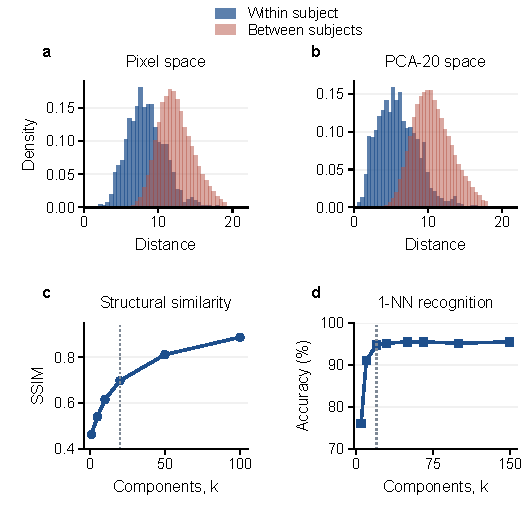
\includegraphics[width=\columnwidth]{fig6_metrics_panels.pdf}
  \caption{Separability and task metrics. (a) Within- and between-subject
  distance distributions in pixel space; (b) the same in PCA-20 space;
  (c) mean SSIM versus $k$; (d) self-excluded 1-NN accuracy using the
  full-data basis. Dashed vertical lines mark $k=20$.}
  \label{fig:metrics}
\end{figure}

\subsection{Runtime and Storage}
Table~\ref{tab:eff} and Fig.~\ref{fig:efftime} compare the two solvers on the
same machine with the same data. The economy SVD needs \nSvdMed{}\,s (median
of three runs; range \nSvdLow{}--\nSvdHigh{}\,s) against \nEighMed{}\,s
(range \nEighLow{}--\nEighHigh{}\,s) for the covariance route, a
\nSpeedup$\times$ speed-up; a second independent run of the same pipeline
reproduced the ordering (\nSvdMedTwo{}\,s versus \nEighMedTwo{}\,s), although
absolute times vary between runs. The gap
is explained by the operation counts: with $n\ll d$ the covariance route
spends $O(d^3)$ on a $d\times d$ eigendecomposition, while the economy SVD
works with the $n\times d$ data and costs $O(nd\min(n,d))$. For these
dimensions, the leading-order ratio $(d/n)^2\approx105$ illustrates the
scale difference, with algorithm-dependent constants omitted. The covariance matrix alone
would occupy \nCovMem{} in float64, compared with \nStorageOrig{} for the
data matrix. These estimates exclude solver workspaces and outputs.

\begin{table}[!t]
  \caption{Solver times: median and range of three runs.
  Array storage estimates assume float64 and exclude workspace.}
  \label{tab:eff}
  \centering
  \footnotesize
  \setlength{\tabcolsep}{4pt}
  \begin{tabular}{@{}lrrr@{}}
    \toprule
    Solver & Median & Range & Array \\
           & (s) & (s) & (MB) \\
    \midrule
    Covariance + eigh & 23.4 & 21.4--24.7 & 134 \\
    Economy SVD & 0.97 & 0.82--1.43 & 13.1 \\
    \bottomrule
  \end{tabular}
  \vspace{3pt}
  \parbox{\columnwidth}{\scriptsize Arrays: covariance matrix $C$
  ($4096\times4096$) and centered data $\tilde X$ ($400\times4096$),
  respectively. These are reference array sizes, not measured peak memory.}
\end{table}


\begin{figure}[tb]
  \centering
  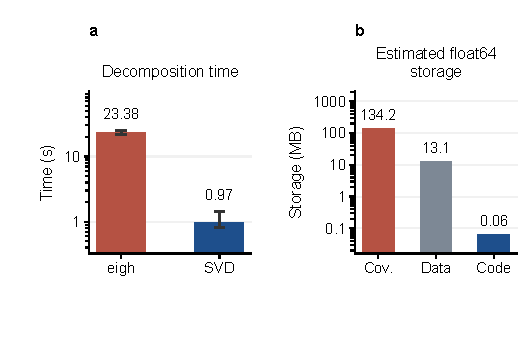
\includegraphics[width=\columnwidth]{fig10_efficiency.pdf}
  \caption{Efficiency at a glance: decomposition time on a log scale with the
  observed range over three runs (left); reference float64 array storage
  for the covariance matrix, centered data, and PCA codes (right).}
  \label{fig:efftime}
\end{figure}

Encoding and reconstruction require approximately $4kd=0.33$ million
floating-point operations per image when multiplication and addition each
count as one operation. The recorded median latency is
\nLatency{}\,ms per image over five passes through the dataset. At $k=20$,
the coefficients require 160 bytes per image in float64, or
\nStorageKB{} for all images, approximately \nCompress$\times$ less than
the original pixel array. Decoding also requires the shared basis and mean.
Including these arrays gives $8(nk+dk+d)=752{,}128$ bytes, approximately
0.752\,MB, for the model and all codes. Thus the coefficient-only reduction
should be distinguished from the complete representation's storage cost.

\subsection{Held-out Evaluation}
\label{sec:heldout}
The fixed \nTrainN/\nTestN{} split evaluates $k=20$ on images excluded
from basis estimation. Test reconstruction MSE rises from \nMSEK{}
to \nTestMSE{} ($+\nMseRise$ relative to the in-sample value), PSNR falls
from \nPSNRK{} to \nTestPSNR{}\,dB and SSIM from \nSsimK{} to \nTestSSIM{};
1-NN accuracy with the training gallery drops from \nAccK{} to \nTestAcc{},
while the within-/between-subject distance ratio is similar
(\nSepPCA{} for the full-data projections versus \nTestSep{} for held-out
projections). All test subjects are represented in the training gallery.
This performance gap combines changes in basis estimation and gallery
size; a single split at one $k$ does not establish generalization to new
identities or validate the full component-count sweep.

\section{Discussion}
Reconstruction and classification favor different component counts.
Increasing $k$ continues to
improve pixel error and SSIM, whereas self-excluded 1-NN accuracy approaches
a plateau near $k=50$. The operating point should therefore reflect the
target metric and the marginal benefit of additional components.

The solver comparison separates representation quality from computational
cost. The two solvers estimate the same leading subspace and produce
numerically equivalent reconstructions in this experiment. The runtime
advantage of economy SVD is consistent with its lower complexity when
$n\ll d$, although the measured speed-up is specific to the implementations
and machine tested.

The lower distance ratio suggests that the retained subspace preserves
relatively more between-subject variation than within-subject variation.
It does not identify the acquisition factors responsible for that change.
The held-out results further restrict the supported classification claim
to new images of known identities under the tested gallery protocol.

\section{Limitations and Future Work}
\label{sec:limits}
Evidence is limited to one small dataset and one fixed split. Repeated
splits with PCA refitted within each training fold would quantify partition
sensitivity; cross-session recordings and unseen identities would test
broader recognition claims.

Timings lack a complete hardware and numerical-library configuration for
cross-machine comparison. Array storage estimates exclude solver
workspaces. Separability pools illumination and expression within subjects;
factor-specific analysis and comparisons with 2-D PCA or kernel PCA could
clarify which variations the linear representation retains.

\section{Conclusion}
This study jointly evaluates reconstruction quality and computational cost
for PCA face reconstruction. With $k=\nK$ components, PCA retains
\nVarKsSum{} of the variance and reduces reconstruction MSE by \nDrop{}
relative to the mean-face baseline. Economy SVD produces numerically
equivalent reconstructions while reducing median decomposition time from
\nEighMed{} to \nSvdMed{}\,s. The results support SVD for this $n\ll d$
setting and show that component selection should reflect the reconstruction
or classification objective. Held-out findings concern new images of known
subjects. The
accompanying code, figures, and recorded experiment output support
reproduction of the analysis.

% 不强制参考文献另起页；末页双栏由 flushend 自动平衡。
\begin{thebibliography}{9}
\label{sec:refs}

\bibitem{jolliffe}
I.~T. Jolliffe, \emph{Principal Component Analysis}, 2nd~ed.
New York, NY, USA: Springer, 2002.

\bibitem{turk}
M.~Turk and A.~Pentland, ``Eigenfaces for recognition,'' \emph{J. Cognitive
Neuroscience}, vol.~3, no.~1, pp.~71--86, 1991.

\bibitem{orl}
The ORL Database of Faces, AT\&T Laboratories Cambridge. [Online]. Available:
\url{http://www.cl.cam.ac.uk/research/dtg/attarchive/facedatabase.html}

\bibitem{sklearn}
F.~Pedregosa \emph{et~al.}, ``Scikit-learn: Machine learning in Python,''
\emph{J. Mach. Learn. Res.}, vol.~12, pp.~2825--2830, 2011.

\bibitem{abdi}
H.~Abdi and L.~J. Williams, ``Principal component analysis,'' \emph{WIREs
Comput. Stat.}, vol.~2, no.~4, pp.~433--459, 2010.

\bibitem{golub}
G.~H. Golub and C.~F. Van~Loan, \emph{Matrix Computations}, 4th~ed.
Baltimore, MD, USA: Johns Hopkins Univ. Press, 2013.

\bibitem{yang}
J.~Yang, D.~Zhang, A.~F. Frangi, and J.-y. Yang, ``Two-dimensional PCA: A new
approach to appearance-based face representation and recognition,'' \emph{IEEE
Trans. Pattern Anal. Mach. Intell.}, vol.~26, no.~1, pp.~131--137, 2004.

\bibitem{scholkopf}
B.~Sch\"olkopf, A.~Smola, and K.-R. M\"uller, ``Nonlinear component analysis
as a kernel eigenvalue problem,'' \emph{Neural Computation}, vol.~10, no.~5,
pp.~1299--1319, 1998.

\bibitem{ssim}
Z.~Wang, A.~C. Bovik, H.~R. Sheikh, and E.~P. Simoncelli, ``Image quality
assessment: From error visibility to structural similarity,'' \emph{IEEE
Trans. Image Process.}, vol.~13, no.~4, pp.~600--612, 2004.

\end{thebibliography}

\end{document}
